\documentclass[../../compsys.tex]{subfiles}
\begin{document}
\raggedbottom
\chapter{L16 — Routing and BGP}
\vfill
\raggedbottom

\section{Quick Review: Forwarding vs. Routing}
Let's quickly review the two main jobs of the network layer from last time.

\subsection{Forwarding: What Each Router Does}
\textbf{Forwarding} is a local operation that happens whenever a packet arrives at a router:
\begin{itemize}
    \item Goal: Figure out which output link to send the packet to
    \item How: Read the destination IP address from the packet header and look it up in the forwarding table
    \item It's fast and happens for every single packet
\end{itemize}

\subsection{Routing: How Forwarding Tables Get Filled}
\textbf{Routing} is a network-wide operation that populates forwarding tables:
\begin{itemize}
    \item Goal: Figure out what should go in each router's forwarding table
    \item How: Run routing algorithms either on a centralized controller or on the routers themselves
    \item It's slower and happens when the network changes
\end{itemize}

\section{How Internet Forwarding Works}
\textit{The Internet uses packet switching with best-effort delivery.}

Remember these key points about Internet forwarding:
\begin{itemize}
    \item Uses packet switching (no virtual circuits or network-layer connections)
    \item Provides best-effort service (no guarantees about delivery or performance)
    \item Each forwarding table entry contains: destination IP prefix + output link
    \item These entries are populated by routing protocols
\end{itemize}

We talked a lot about forwarding tables in the last lecture, but we didn't really discuss how big they are. Today we'll get more concrete about forwarding table sizes and how routing works.

\section{Every Router Knows About Every Destination}
\textit{Every router on the Internet can reach every public IP address.}

Let's say there's an end-system somewhere with IP address 8.0.0.1. Here's the amazing part:

\begin{itemize}
    \item Every router on the Internet has an entry in its forwarding table that matches 8.0.0.1
    \item That entry tells the router which output link to use to get packets closer to 8.0.0.1
    \item This is true for ANY public Internet IP address, not just 8.0.0.1
\end{itemize}

This is what makes global connectivity possible - every router knows how to reach every destination!

\section{First-Hop Routers: Where It All Starts}
\textit{Some routers have a special job - they're the first ones to handle packets from local networks.}

\begin{center}
    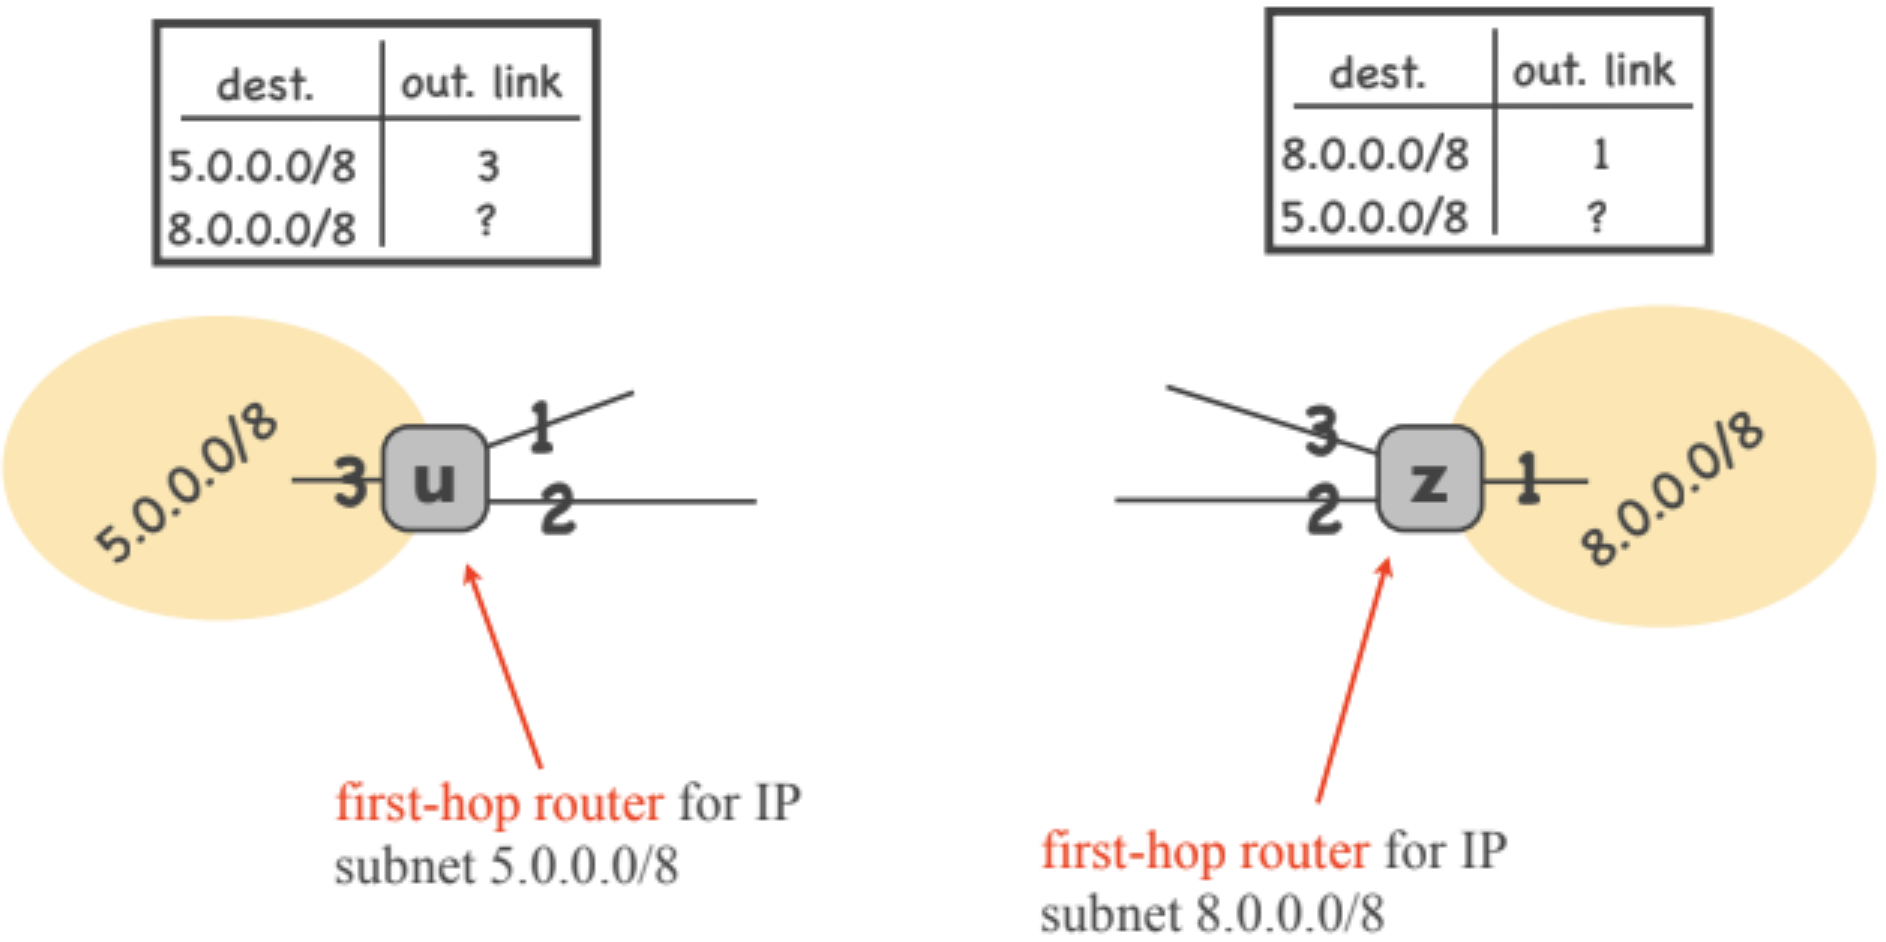
\includegraphics[width=0.6\textwidth]{images/hop-router.png}
\end{center}

Let's look at an example with two IP subnets:
\begin{itemize}
    \item Left subnet: uses IP prefix 5.0.0.0/8
    \item Right subnet: uses IP prefix 8.0.0.0/8
\end{itemize}

Each subnet connects to a router:
\begin{itemize}
    \item Router u connects to the left subnet (5.0.0.0/8)
    \item Router z connects to the right subnet (8.0.0.0/8)
\end{itemize}

We call these \textbf{first-hop routers} because they're the first routers to handle packets coming from their local subnets.

\subsection{What First-Hop Routers Know Automatically}
Each first-hop router automatically knows about its own local subnet:

\textbf{Router u knows:}
\begin{itemize}
    \item "Any packet for 5.0.0.0/8 goes out my link 3 (to the local subnet)"
    \item The network administrator configures this when setting up the router
\end{itemize}

\textbf{Router z knows:}
\begin{itemize}
    \item "Any packet for 8.0.0.0/8 goes out my link 1 (to the local subnet)"
    \item This is also configured manually by the administrator
\end{itemize}

\subsection{The Big Question: What About Foreign Subnets?}
But here's the problem: how does router u learn to forward packets to router z's subnet (8.0.0.0/8)? And how does router z learn about router u's subnet (5.0.0.0/8)?

The network administrator can't manually configure every possible destination - there are millions of them!

\textbf{The answer: A routing protocol.}

Routing protocols are software systems that automatically figure out how to reach all destinations and populate the forwarding tables accordingly.

\section{How Routing Protocols Work: A Simple Example}
\textit{Let's see what happens when routers need to figure out the best paths to each other.}

Suppose we have 3 routers: u, v, and z. When these routers participate in a routing protocol, their goal is to learn the best path to reach each other.

\begin{center}
    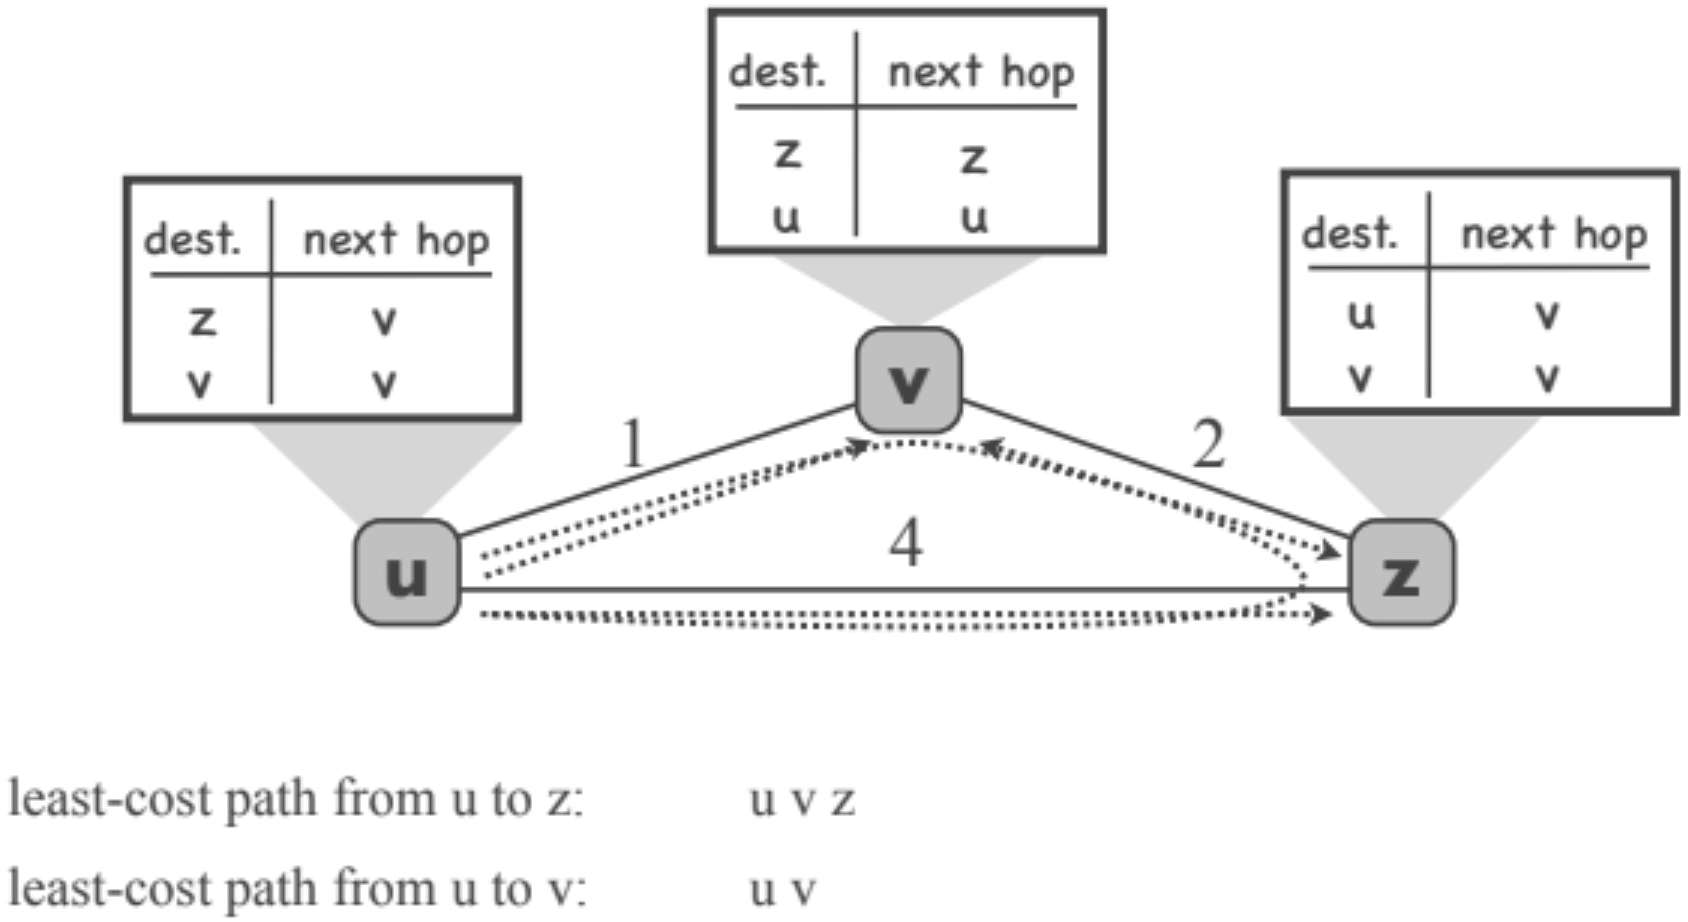
\includegraphics[width=0.6\textwidth]{images/example-table-routers.png}
\end{center}

Let's think about router u. It needs to answer these questions:
\begin{itemize}
    \item "When I want to send a packet to router z, should I send it directly or through router v?"
    \item "When I want to send a packet to router v, what's the best way?"
\end{itemize}

The other routers (v and z) need to answer similar questions about reaching their destinations.

\subsection{What Does "Best Path" Mean?}
\textit{To pick the best path, we need to define what "best" means.}

Each link in the network has a \textbf{cost} that represents how "bad" or expensive it is to use that link. The cost could be based on:
\begin{itemize}
    \item How long it takes for signals to travel across the link (propagation delay)
    \item How much money it costs to send traffic over that link
    \item How congested the link is
    \item Some other cost metric that network administrators choose
\end{itemize}

The cost of a \textbf{path} is simply the sum of the costs of all links in that path. The \textbf{best path} from one router to another is the path with the lowest total cost—this is called the \textbf{least-cost path}.

\textbf{Important note:} In our examples, a link's cost is the same in both directions. In reality, links can have different costs in each direction, but we'll keep it simple for now.

\section{Working Out the Best Paths: Step by Step}
\textit{Let's figure out the best paths for router u in our example.}

Looking at the network diagram, let's calculate the costs:

\begin{center}
    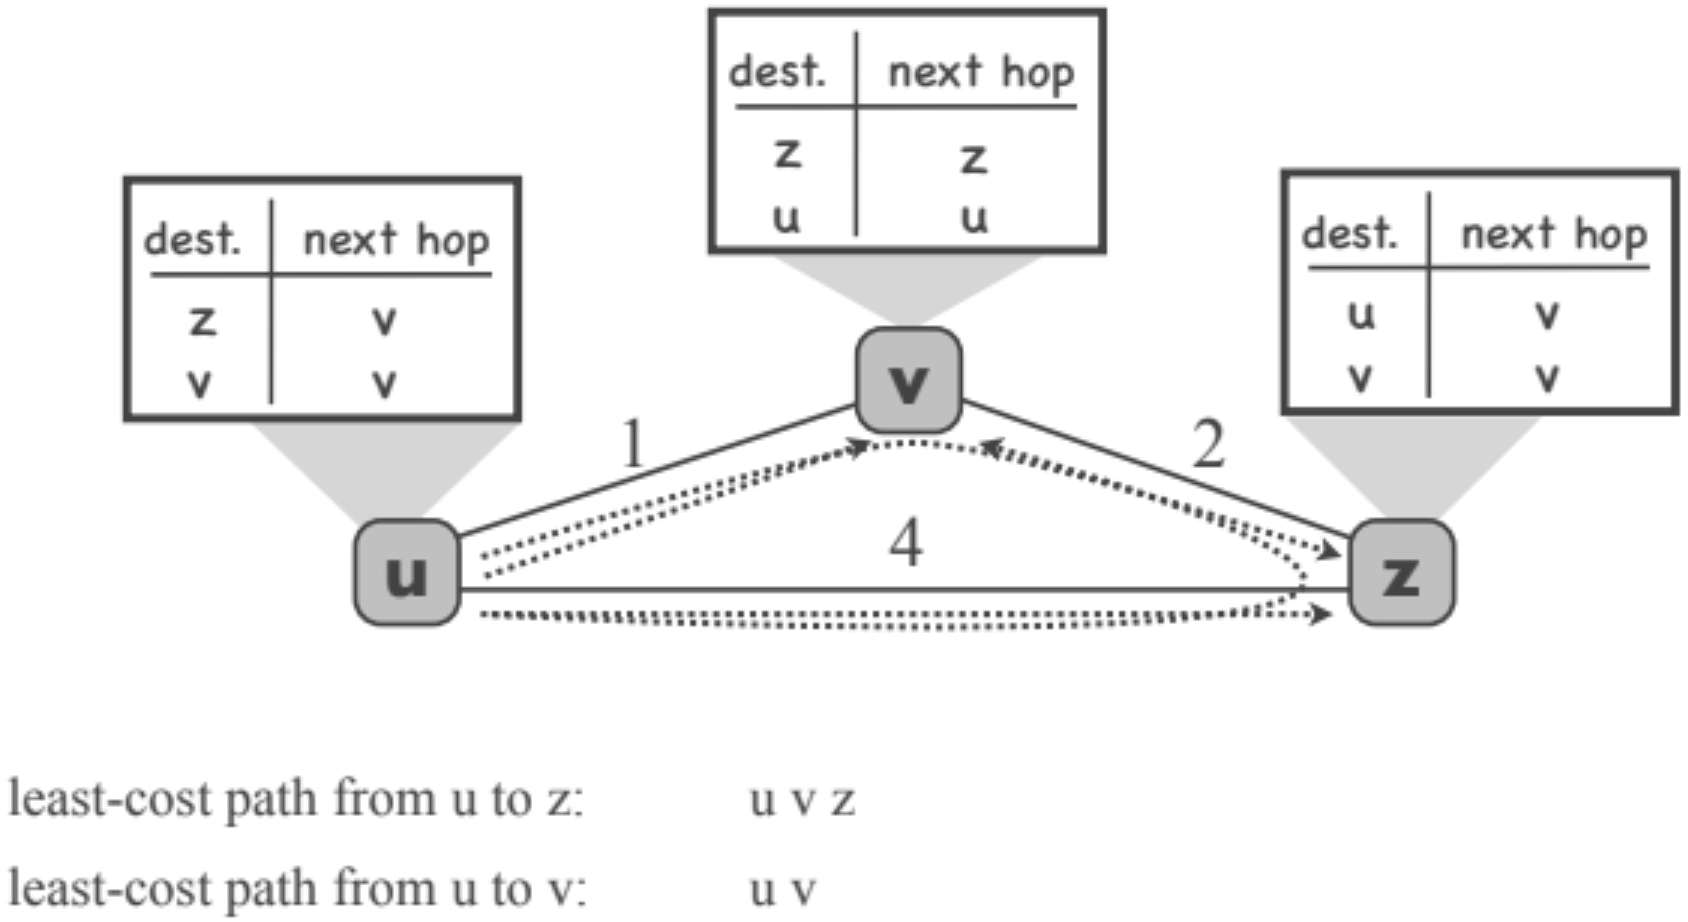
\includegraphics[width=0.6\textwidth]{images/example-table-routers.png}
\end{center}

\subsection{From Router u to Router z}
Router u has two options to reach router z:\\[10px]
\textbf{Option 1: Direct path}
\begin{itemize}
    \item Go directly from u to z
    \item Cost = 4
\end{itemize}

\textbf{Option 2: Indirect path through v}
\begin{itemize}
    \item Go from u to v, then from v to z
    \item Cost = 1 + 2 = 3
\end{itemize}

Since 3 $<$ 4, the best path is the indirect one through router v.
Therefore, router u should send packets destined for z to router v as the next hop.

\subsection{From Router u to Router v}
Router u has two options to reach router v:

\textbf{Option 1: Direct path}
\begin{itemize}
    \item Go directly from u to v
    \item Cost = 1
\end{itemize}

\textbf{Option 2: Indirect path through z}
\begin{itemize}
    \item Go from u to z, then from z to v
    \item Cost = 4 + 2 = 6
\end{itemize}

Since 1 $<$ 6, the best path is the direct one.
Therefore, router u should send packets destined for v directly to v.

\section{Link-State Routing Algorithms}
\textit{This is the first major family of routing algorithms.}

The process we just did by hand is an example of a \textbf{link-state routing algorithm}. Here's the general idea:
\begin{itemize}
    \item \textbf{Input:} A complete map of the network—all the routers and the costs of all links connecting them.
    \item \textbf{Output:} The least-cost path from one starting router to every other router in the network.
\end{itemize}

The most famous link-state routing algorithm is called \textbf{Dijkstra's algorithm}.

\subsubsection{Why It's Called "Centralized"}
Link-state routing algorithms are sometimes called \textbf{"centralized"} algorithms.
\begin{itemize}
    \item[-] Each router first gets a copy of the entire network map.
    \item[-] Once a router has the full map, it can calculate the best paths to all other routers \textbf{by itself}, without any more communication.
    \item[-] Each router runs the algorithm independently on its own copy of the map.
\end{itemize}

\section{Distance-Vector Routing Algorithms}
\textit{This is the second major family of routing algorithms, and it works very differently.}

Instead of knowing the whole map, routers in a \textbf{distance-vector} algorithm only know about their immediate neighbors. They work together in rounds to figure out the best paths.

\subsection{The Setup: What Each Router Knows Initially}
Let's use our 3-router example again. In a distance-vector algorithm, each router starts by creating a table with the costs to its direct neighbors.

\begin{center}
    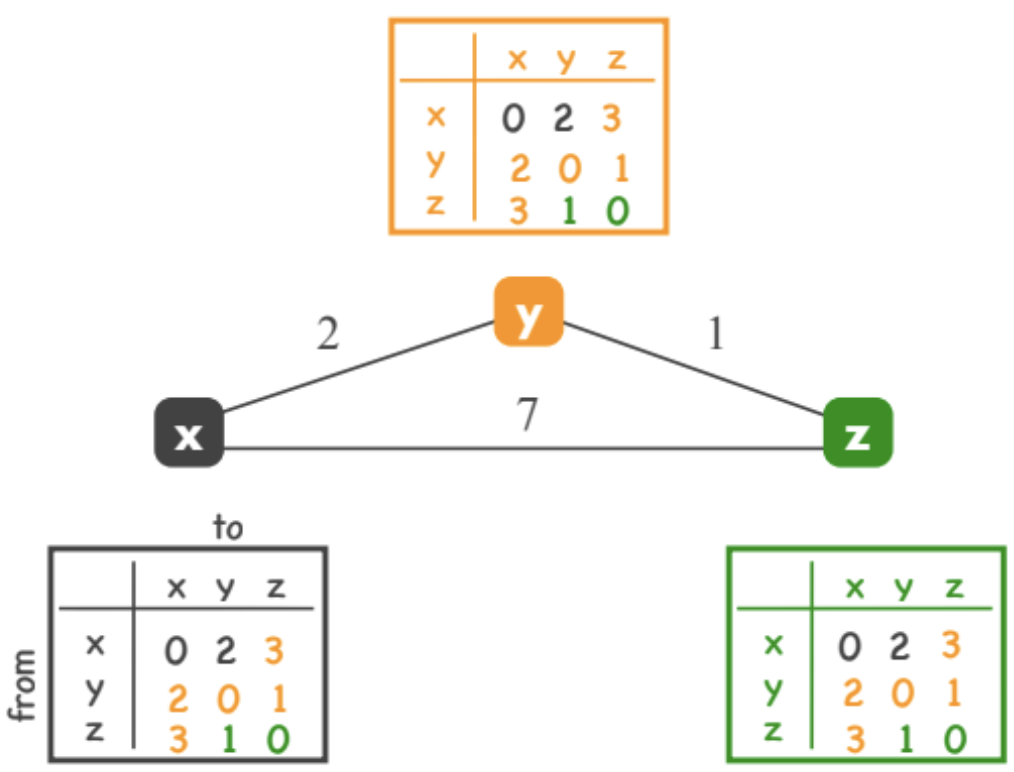
\includegraphics[width=0.6\textwidth]{images/dijkstra-example.png}
\end{center}
\begin{minipage}{0.3\textwidth}
\textbf{Router x knows:}
\begin{itemize}
    \item Cost to itself (x) is 0
    \item Cost to neighbor y is 2
    \item Cost to neighbor z is 7
\end{itemize}
\end{minipage}
\begin{minipage}{0.3\textwidth}
\textbf{Router y knows:}
\begin{itemize}
    \item Cost to neighbor x is 2
    \item Cost to itself (y) is 0
    \item Cost to neighbor z is 1
\end{itemize}
\end{minipage}
\begin{minipage}{0.3\textwidth}
\textbf{Router z knows:}
\begin{itemize}
    \item Cost to neighbor x is 7
    \item Cost to itself (z) is 0
    \item Cost to neighbor y is 1
\end{itemize}
\end{minipage}\\[10px]
They don't know about any indirect paths yet!

\subsection{Round 1: Exchanging Information}
In the first round, all routers send their tables to their immediate neighbors.
\begin{itemize}
    \item Router x sends its table to y and z.
    \item Router y sends its table to x and z.
    \item Router z sends its table to x and y.
\end{itemize}

\subsection{Round 1: Updating the Tables}
Now, each router looks at the information it received from its neighbors and asks: "Can my neighbors get me somewhere cheaper than I can get there myself?"

\textbf{Let's look at router x:}
\begin{itemize}
    \item Router x knows it can get to z with a direct cost of 7.
    \item But it just learned from router y that "y can get to z with a cost of 1".
    \item Router x knows it can get to y with a cost of 2.
    \item So, x thinks: "I can get to y (cost 2), and y can get to z (cost 1). The total cost is 2 + 1 = 3."
    \item Since 3 is cheaper than 7, router x updates its table: "The new best cost to reach z is 3, by going through y."
\end{itemize}

\textbf{Now let's look at router z:}
\begin{itemize}
    \item Router z knows it can get to x with a direct cost of 7.
    \item But it just learned from router y that "y can get to x with a cost of 2".
    \item Router z knows it can get to y with a cost of 1.
    \item So, z thinks: "I can get to y (cost 1), and y can get to x (cost 2). The total cost is 1 + 2 = 3."
    \item Since 3 is cheaper than 7, router z updates its table: "The new best cost to reach x is 3, by going through y."
\end{itemize}

Router y doesn't find any new cheaper paths in this round because its direct connections are already the best.

\subsection{Round 2: The Final Check}
In the second round, all routers exchange their new, updated tables with their neighbors again.

This time, when they check the new information, they find that they can't improve their paths any further. Everyone already has the best possible path.

When no router can find a cheaper path, the algorithm is done! Each router has now successfully computed the least-cost path to every other router in the network.

\section{The Bellman-Ford Algorithm}
\textit{The specific distance-vector algorithm we just learned has a name.}

The particular distance-vector routing algorithm we discussed is called the \textbf{Bellman-Ford algorithm}.

\subsection{How Bellman-Ford Works}
Here's the process in summary:
\begin{itemize}
    \item \textbf{Step 1:} All neighbors exchange their routing tables
    \item \textbf{Step 2:} Each router checks whether it can use the new information to improve its current paths
    \item \textbf{Step 3:} If improvements are found, update the table
    \item \textbf{Repeat:} Continue until no router can improve its paths any further
\end{itemize}

The algorithm ends when no improvement is possible, which means everyone has found their optimal paths.

\section{Link-State vs. Distance-Vector: The Big Picture}
\textit{Both approaches solve the same problem but in very different ways.}

We've now learned about two major families of routing algorithms:
\begin{itemize}
    \item \textbf{Link-state algorithms} (like Dijkstra's)
    \item \textbf{Distance-vector algorithms} (like Bellman-Ford)
\end{itemize}

\textbf{The goal is the same for both:} Compute the least-cost path from each router to every other router in the network.


\section{Which Approach Is Better?}
\textit{Each approach has its own advantages and trade-offs.}

\subsection{Link-State Advantages: Speed}
\textbf{Link-state converges faster:}
\begin{itemize}
    \item[-] Each router starts with the full picture of the network
    \item[-] Once a router has the complete map, it can calculate all paths immediately
    \item[-] The computation time can be reduced by using faster computers
    \item[-] No waiting for information to propagate through multiple rounds
\end{itemize}

Think of it this way: if you have the complete map, you can plan the fastest route right away.

\subsection{Distance-Vector Advantages: Efficiency}
\textbf{Distance-vector uses less bandwidth:}
\begin{itemize}
    \item[-] Each router only talks to its immediate neighbors
    \item[-] The number of messages per round stays constant regardless of network size
    \item[-] No need to flood the entire network with information
    \item[-] More efficient use of network resources
\end{itemize}

\section{Bringing It All Together: How Routing Completes Forwarding Tables}
\textit{Let's see how routing protocols solve the real problem we started with.}

Remember our example from the beginning? Router u knew how to handle packets for its local subnet (5.0.0.0/8) but didn't know what to do with packets destined for 8.0.0.0/8.

\begin{center}
    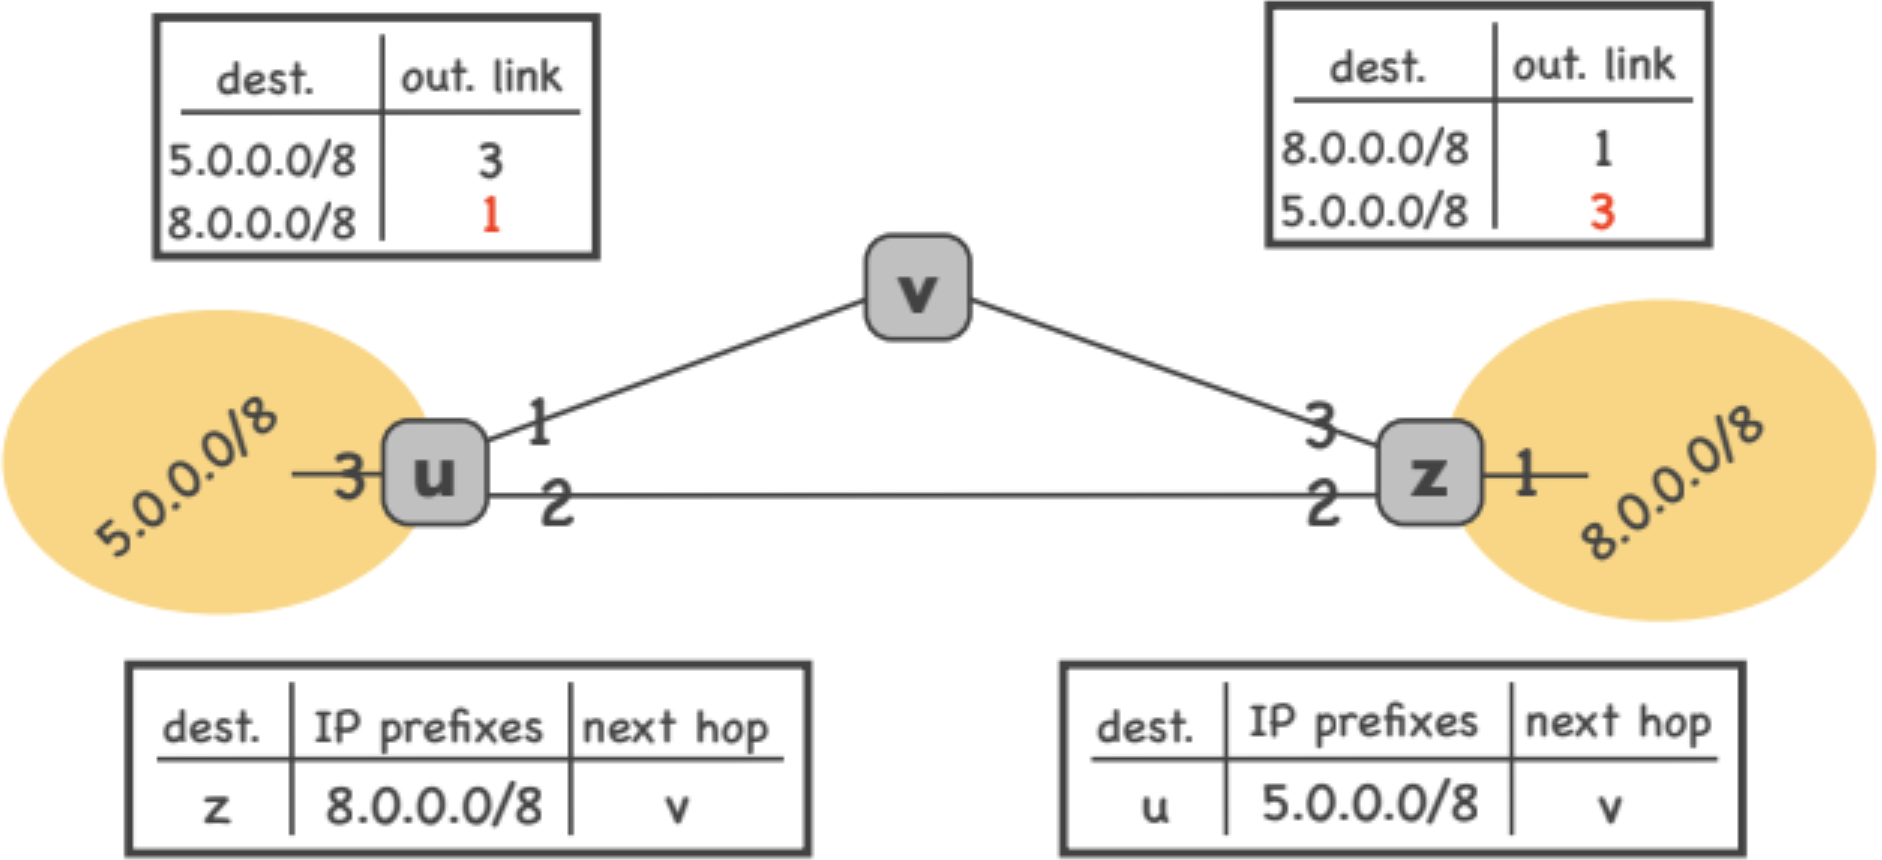
\includegraphics[width=0.6\textwidth]{images/example.png}
\end{center}

Here's how a routing protocol solves this problem:\\
\begin{minipage}[htp]{0.5\textwidth}
    \textbf{Step 1: Routers Advertise What They Own}
    Each router announces which IP prefixes it "owns":
    \begin{itemize}
        \item[-] Router u advertises: "I own IP prefix 5.0.0.0/8"
        \item[-] Router z advertises: "I own IP prefix 8.0.0.0/8"
    \end{itemize}
    \end{minipage}
    \begin{minipage}[htp]{0.5\textwidth}
 \textbf{Step 2: Routing Protocol Finds Best Paths}
    Router u, router v, and router z all participate in a routing protocol (could be Dijkstra, Bellman-Ford, or any other routing algorithm). Through this protocol:
    \begin{itemize}
        \item[-] Router u learns that the best next hop to reach router z is router v
        \item[-] Router u also learns that router z owns IP prefix 8.0.0.0/8
    \end{itemize}
    \end{minipage}\\ 
    \textbf{Step 3: Complete the Forwarding Table}
Router u combines this information:
\begin{itemize}
    \item "To reach 8.0.0.0/8, I need to get to router z"
    \item "To reach router z, my best next hop is router v"
    \item "Router v is reachable through output link 1"
    \item \textbf{Conclusion:} "Map IP prefix 8.0.0.0/8 to output link 1"
\end{itemize}

Similarly, router z learns that:
\begin{itemize}
    \item The best next hop to reach router u is router v
    \item Router u owns IP prefix 5.0.0.0/8
    \item \textbf{Conclusion:} "Map IP prefix 5.0.0.0/8 to output link 3"
\end{itemize}

Now both routers have complete forwarding tables and can route packets anywhere!


\section{The Reality Check: Internet Routing Challenges}
\textit{The algorithms we've learned work great in theory, but the real Internet is much more complex.}

Designing a routing algorithm for the entire Internet faces some serious challenges:

\subsection{Challenge 1: Scale}
The Internet is \textbf{massive}:
\begin{itemize}
    \item Millions of routers worldwide
    \item Millions of IP subnets to track
    \item Constant changes as networks go up and down
\end{itemize}

\textbf{Why our simple algorithms won't work:}
\begin{itemize}
    \item \textbf{Link-state} would cause flooding disasters - imagine every router trying to tell every other router about its links!
    \item \textbf{Distance-vector} would never converge - it would take too many rounds for information to propagate across millions of routers
    \item Forwarding tables would be enormous - one entry for every IP subnet in the world
\end{itemize}

\subsection{Challenge 2: Administrative Autonomy}
Different parts of the Internet are owned by different organizations:
\begin{itemize}
    \item Internet Service Providers (ISPs) like Comcast,Swisscom
    \item Universities like EPFL
    \item Companies like Google, Facebook, Amazon
    \item Government networks
\end{itemize}

\textbf{The problems this creates:}
\begin{itemize}
    \item ISPs may not want to do least-cost routing (they have business reasons for their choices)
    \item ISPs want to hide their internal network details from competitors
    \item Different organizations have different policies about who can send traffic through their networks
\end{itemize}
\newpage
\section{The Internet's Solution: Hierarchical Routing}
The Internet addresses these challenges through \textbf{hierarchy}: dividing into separate networks called \textbf{Autonomous Systems} (ASes).

\subsection{Autonomous Systems}
An AS is a collection of routers under single administrative control (e.g., ISP network, university network, company network). Each AS gets a unique AS number.

\subsection{Two-Level Routing}
\textbf{Intra-AS routing:} Within each AS, routers run their chosen algorithm (Dijkstra, Bellman-Ford, etc.)

\textbf{Inter-AS routing:} Between ASes, border routers use BGP to exchange routes

\subsection{Benefits}
\textbf{Scale:} Thousands of small algorithms instead of one massive algorithm

\textbf{Autonomy:} Each AS controls its own routing policies and can hide internal details

\section{Examples of Intra-AS Routing}
\textit{Different ASes can choose different routing algorithms for their internal networks.}\\[10px]
\textbf{AS 1 might choose:}
\begin{itemize}
    \item Dijkstra's algorithm for fast convergence
    \item Link costs based on bandwidth and delay
\end{itemize}

\textbf{AS 2 might choose:}
\begin{itemize}
    \item Bellman-Ford algorithm to save bandwidth
    \item Link costs based on monetary cost
\end{itemize}

Each AS makes its own decision based on its specific needs and constraints.

\section{A Concrete Example: How an AS Works}
Consider an AS that has 4 routers, each providing connectivity to 1 IP subnet:

\begin{center}
    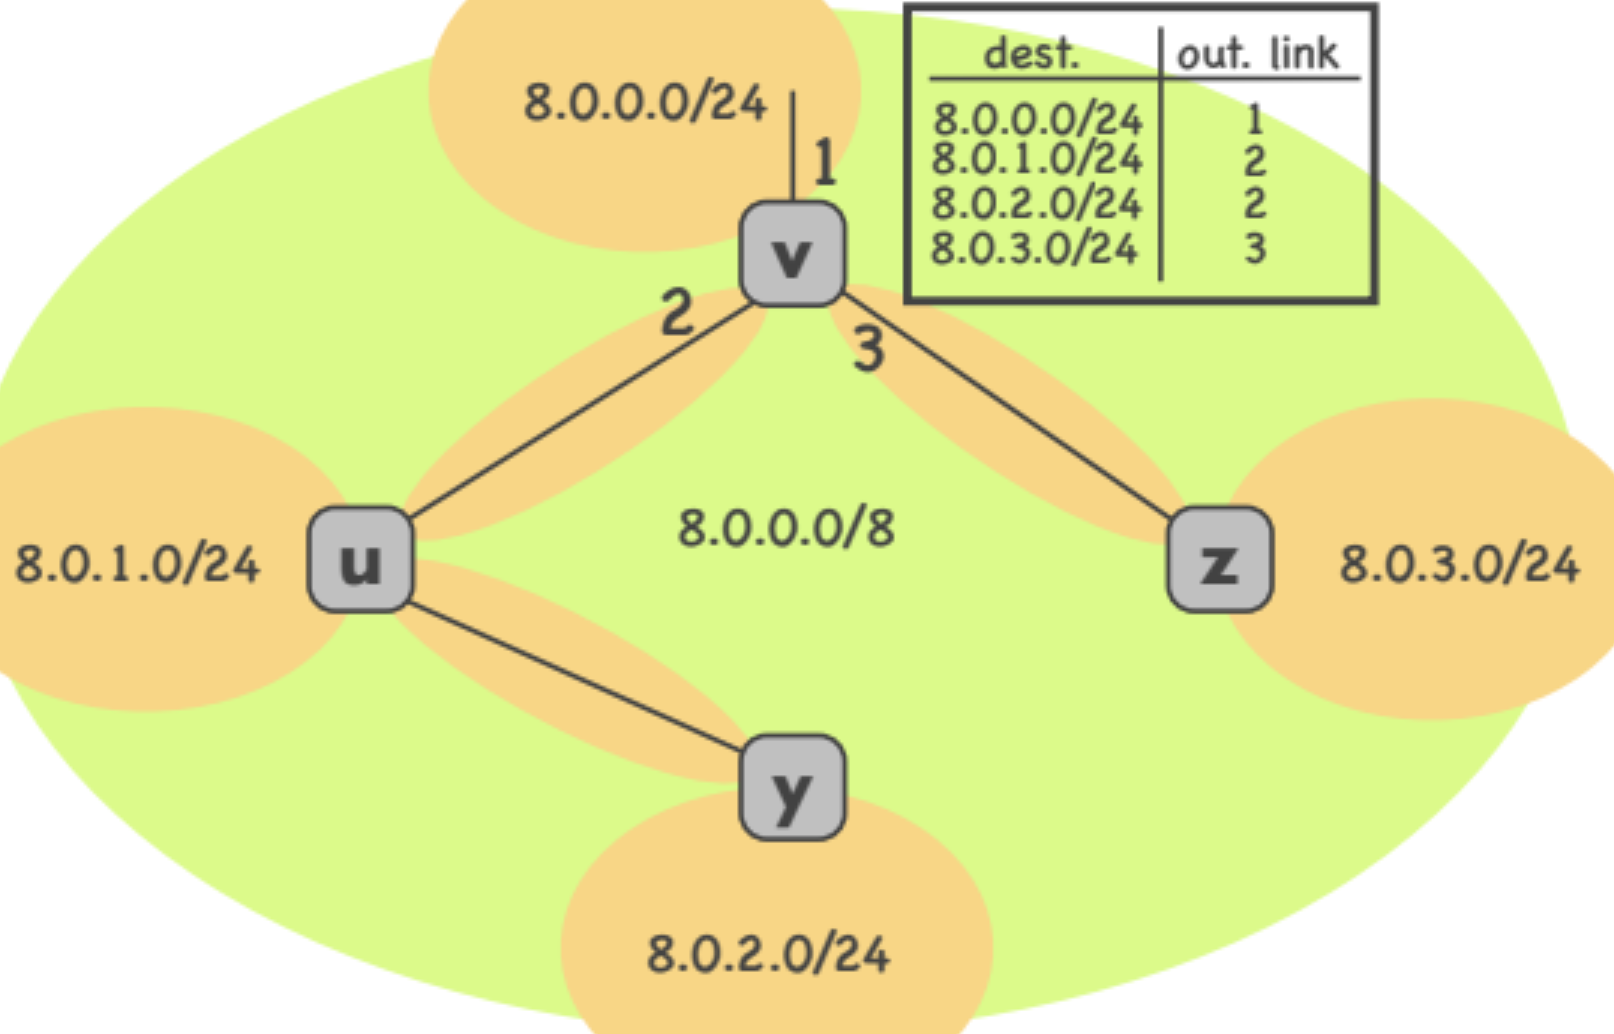
\includegraphics[width=0.6\textwidth]{images/example-as.png}
\end{center}

\subsection{Step 1: Learn About Local Destinations}
Each of the 4 routers must discover the best path to each local router and subnet. They achieve this by participating in an intra-AS routing protocol (like Dijkstra or Bellman-Ford).

\subsection{Foreign Destinations}
Each router must also learn routes to foreign ASes, but \textbf{not} to every individual subnet in those ASes.

\begin{center}
    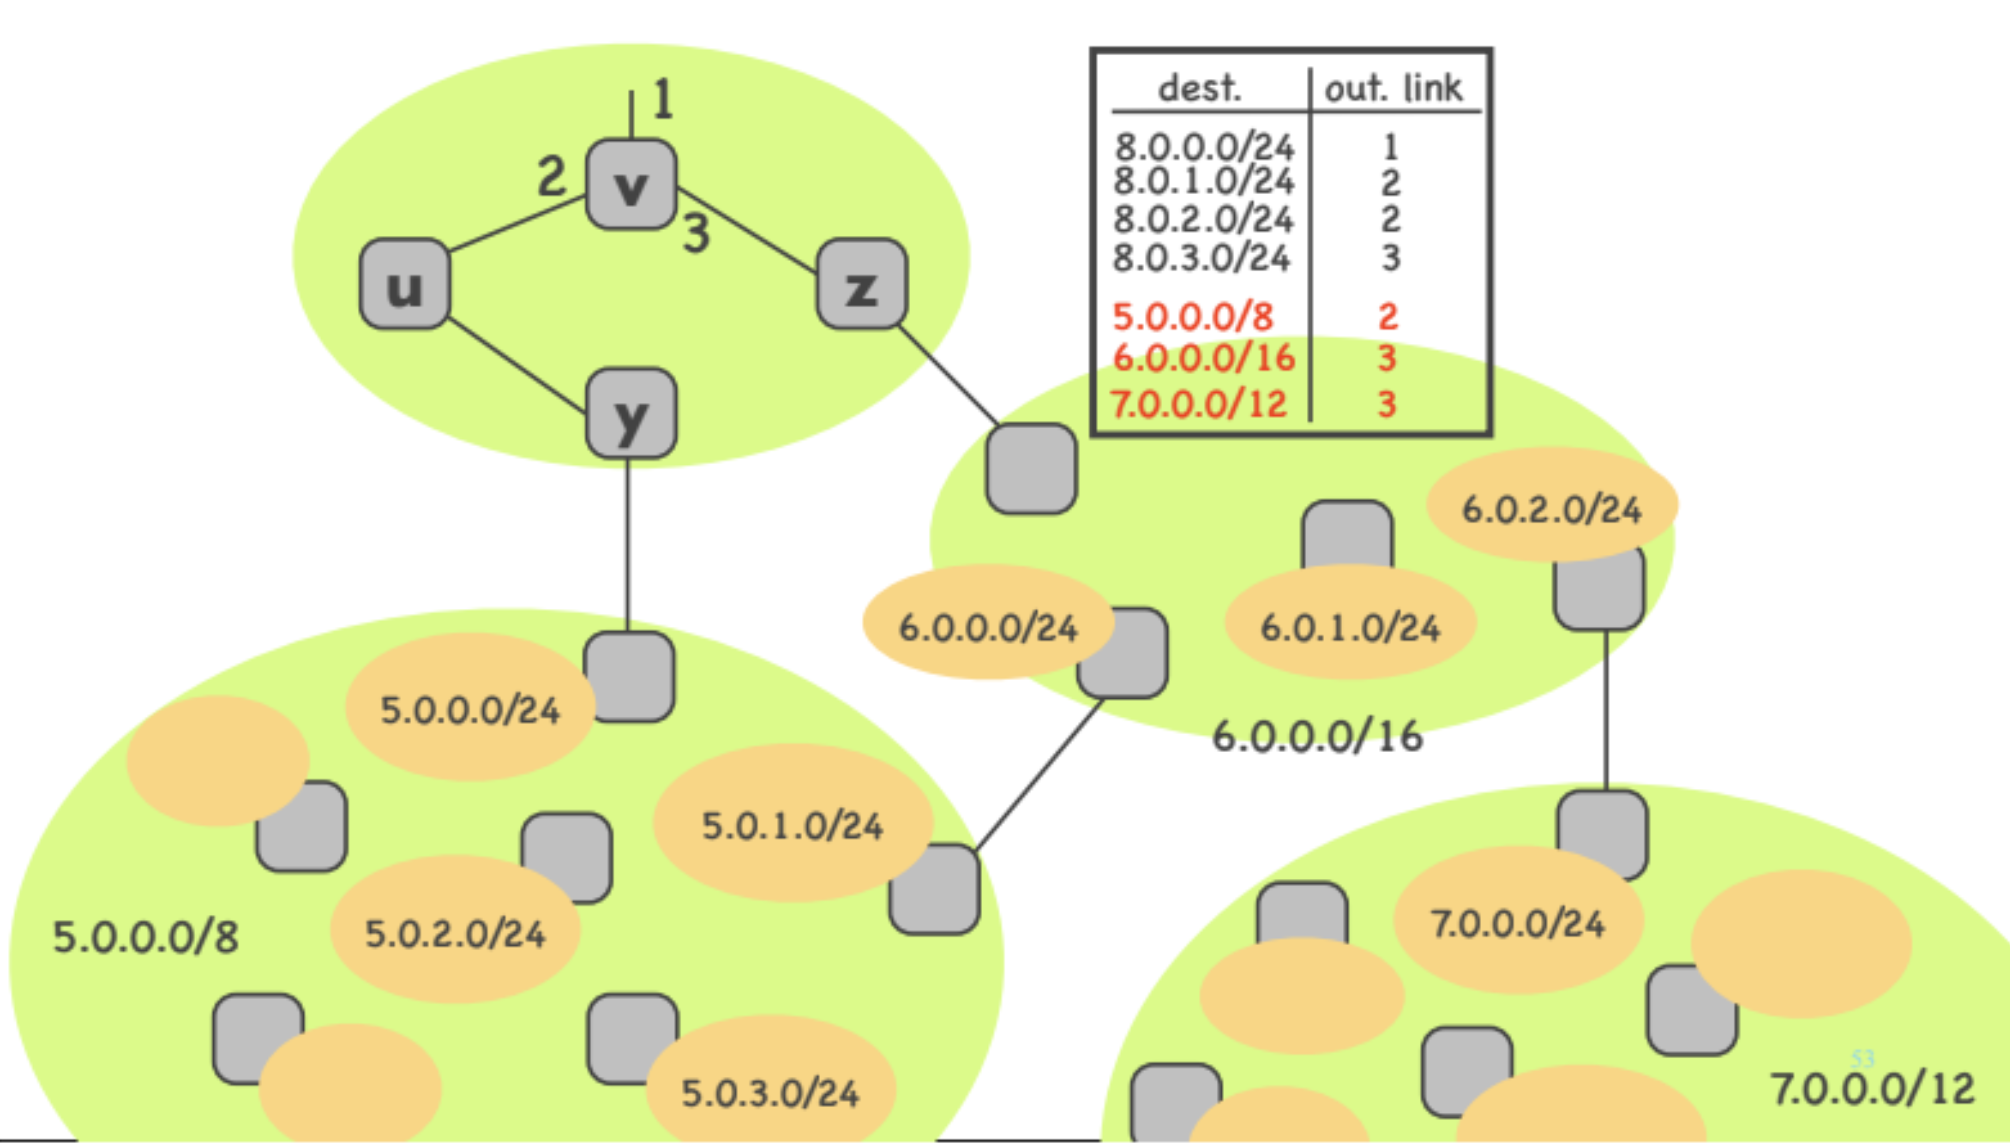
\includegraphics[width=0.6\textwidth]{images/example-as-2.png}
\end{center}

Router v needs only 1 entry for each of the 3 foreign ASes, not separate entries for every subnet within those ASes. This dramatically reduces forwarding table sizes.

\section{Border Routers and BGP}
Border routers sit at the "edge" of each AS and handle communication between different ASes.

\begin{center}
    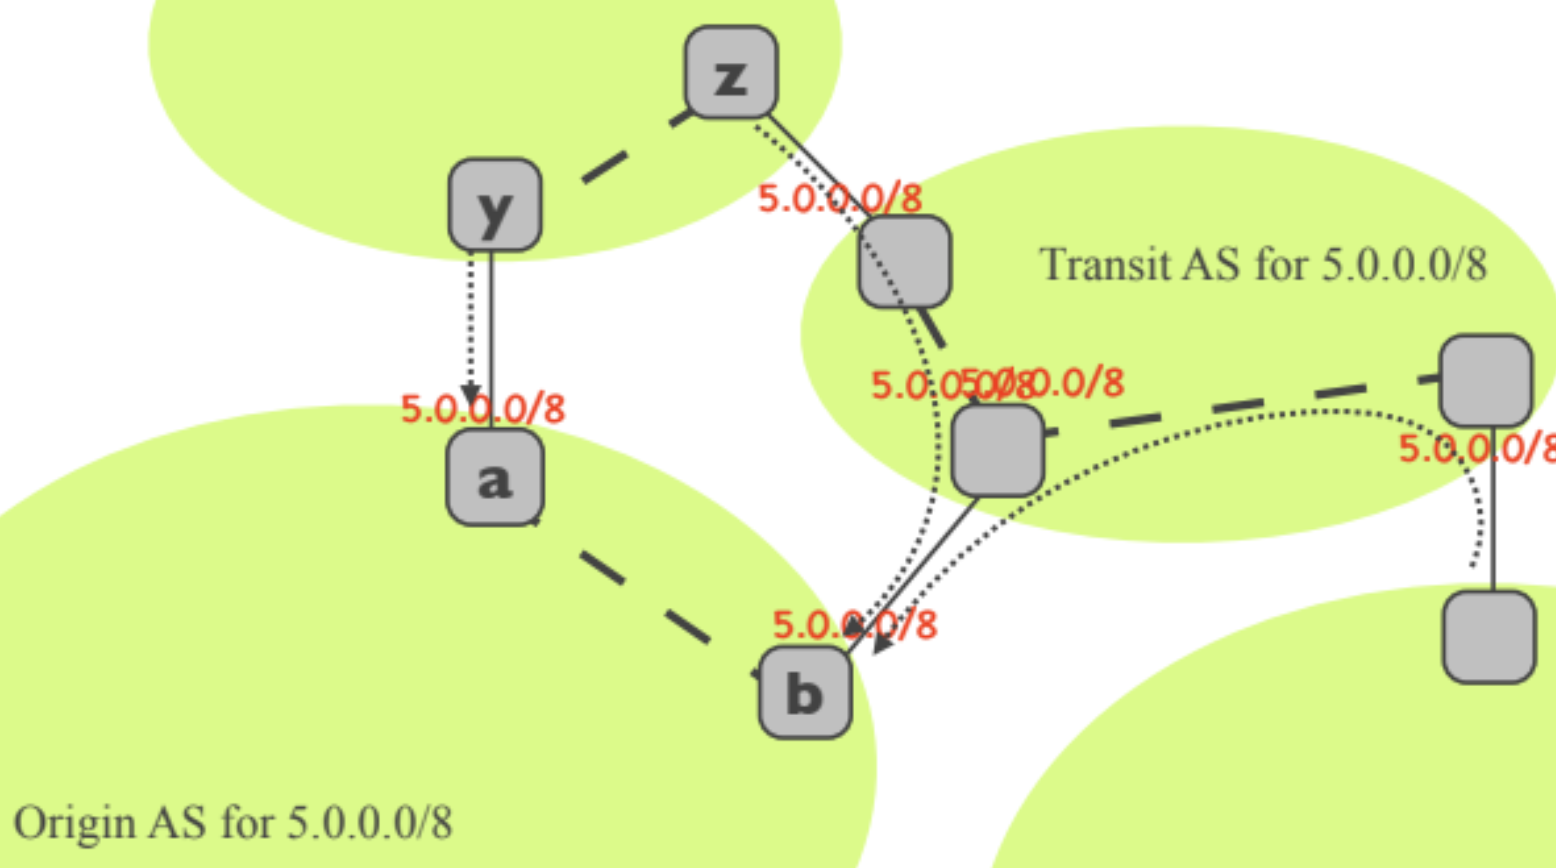
\includegraphics[width=0.45\textwidth]{images/example-as-3.png}
\end{center}

All border routers participate in \textbf{Border Gateway Protocol (BGP)}, a variant of Bellman-Ford. Through BGP, each border router:
\begin{itemize}
    \item Advertises prefixes from its own AS to neighbors
    \item Learns routes to foreign prefixes
\end{itemize}

\subsection{BGP Example}
\begin{itemize}
    \item Bottom left AS aggregates local subnets into 5.0.0.0/8 (becomes the "origin AS")
    \item Border routers a and b advertise "route to 5.0.0.0/8" to their neighbors
    \item Top right AS decides to do transit, propagating the route further
    \item Eventually all ASes learn how to reach 5.0.0.0/8
\end{itemize}

\section{How Non-Border Routers Learn External Routes}
Router v (not a border router):\\
\begin{minipage}[htp]{0.5\textwidth}
\begin{itemize}
    \item Learns local routes from other local routers (intra-AS routing)
    \item Learns foreign routes from border routers y and z
    \item Chooses least-cost route when multiple options exist
\end{itemize}
\end{minipage}
\begin{minipage}[htp]{0.5\textwidth}
\begin{center}
    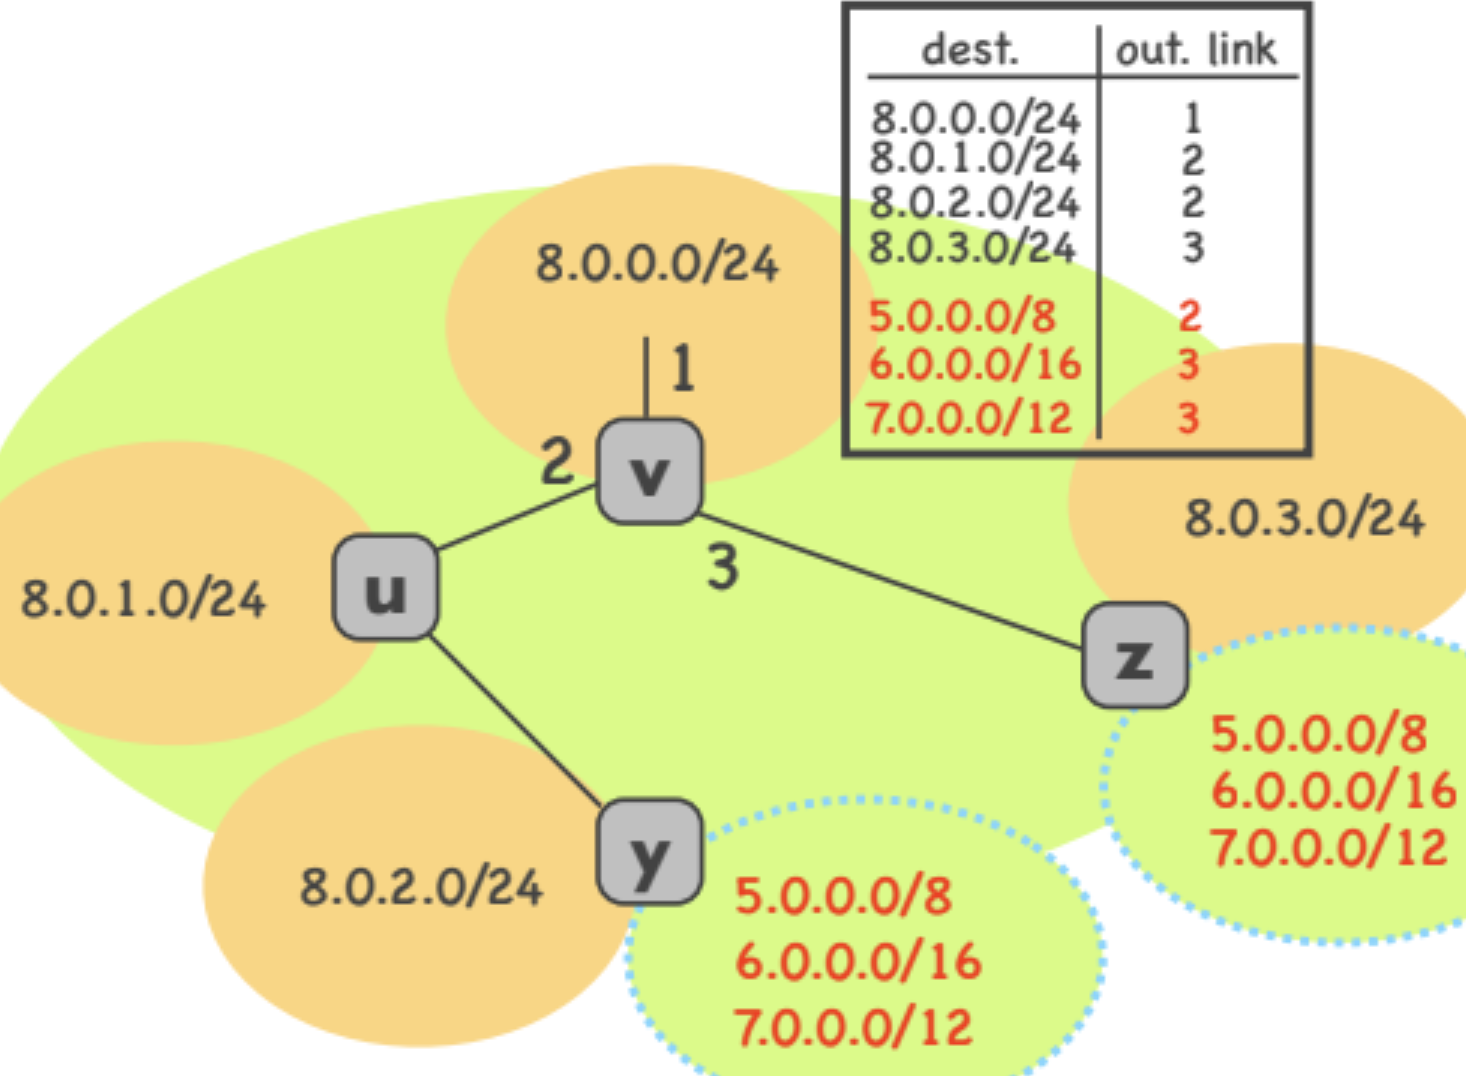
\includegraphics[width=0.8\textwidth]{images/example-as-4.png}
\end{center}
\end{minipage}



\section{Internet Routing Summary}
\subsection{Intra-AS Routing}
\begin{itemize}
    \item \textbf{Participants:} All routers in the same AS
    \item \textbf{Protocols:} OSPF, RIP, others (each AS chooses)
    \item \textbf{Goal:} Propagate routes within local AS
\end{itemize}

\subsection{Inter-AS Routing}
\begin{itemize}
    \item \textbf{Participants:} Border routers between ASes
    \item \textbf{Protocol:} BGP (universal - only one protocol used)
    \item \textbf{Goal:} Propagate routes between ASes
\end{itemize}


\subsubsection{Internet Architecture Foundation}
The Internet's network layer rests on two components:
\begin{itemize}
    \item \textbf{IP:} Specifies forwarding, packet format, addressing
    \item \textbf{BGP:} Inter-domain routing protocol enabling global connectivity
\end{itemize}

\end{document}